\chapter{Thí nghiệm}
\justifying

\setlength{\parindent}{6.5ex}
\label{Chapter4}
\graphicspath{{Chapter4/Chapter4Figs}}
\textit{Trong chương này, chúng tôi trình bày các kết quả thí nghiệm nhằm đánh giá những nội dung trình bày ở chương \ref{Chapter3}. Bộ dữ liệu được dùng để tiến hành các thí nghiệm là bộ MovieLens-20M \cite{Ml20M} và Million Song Dataset \cite{MSD}; bên cạnh đó, độ đo được sử dụng để đánh giá khả năng đưa ra gợi ý của mô hình là Normalized Discounted Cumulative Gain (NDCG) và  Recall. Kết quả thí nghiệm cho thấy mô hình do chúng tôi cài đặt đạt được kết quả xấp xỉ so với kết quả được công bố trong bài báo \cite{mvae}. 
Ngoài ra, chúng tôi còn thực hiện các thí nghiệm     để làm rõ các lý thuyết được đưa ra ở chương trước đó.
Cụ thể chúng tôi thực hiện các thí nghiệm kiểm chứng việc ảnh hưởng của dữ liệu đầu vào trong bài toán xây dưng hệ thống gợi ý sản phẩm;
Và thí nghiệm để làm rõ được sự đánh đổi giữa khả năng mô hình hóa của dữ liệu và việc đặc trưng ẩn tuân theo phân phối xác suất được giả định trong bài toán. 
Bên cạnh đó, các kết quả thí nghiệm cũng chứng tỏ mô hình "Variational Auto-Encoder" có khả đưa ra các gợi ý sản phẩm phù hợp hơn so với mô hình "Auto-Encoder" cơ bản, đặc biệt là trong trường hợp dữ liệu tương tác của người dùng thưa.
}


\section{Tập dữ liệu sử dụng}
\label{chap4sec1}
Chúng tôi tiến hành thí nghiệm trên các tập dữ liệu vừa và lớn ở các lĩnh vực khác nhau là MovieLens-20M \cite{Ml20M} 
và Million Song Dataset (MSD) \cite{MSD}; đây là các tập dữ liệu thường được dùng cho bài toán xây dựng hệ thống gợi ý
với hướng tiếp cận ``Collaborative Filtering''. 
\begin{itemize}
    \item Tập dữ liệu MovieLens-20M bao gồm dữ liệu đánh giá của 138,000 người dùng với khoảng 27,000 bộ phim,
    với 20 triệu đánh giá.
    \item Tập dữ liệu Million Song Dataset bao gồm dữ liệu tương tác (số lượt nghe) của khoảng 1 triệu người dùng và hơn 300,000 bài hát, với hơn 48 triệu tương tác.
\end{itemize}

Để có thể đánh giá kết quả đạt được so với kết quả trong bài báo \cite{mvae} một cách tốt nhất,
chúng tôi thực hiện các bước tiền xử lí được các tác giả mô tả trong bài báo \cite{mvae}.
\begin{itemize}
    \item Tập dữ liệu MovieLens-20M: chúng tôi giữ lại những người dùng đã đánh giá ít nhất 5 bộ phim trở lên. 
    \item Tập dữ liệu Million Song Dataset: chúng tôi chỉ giữ lại những bài hát được nghe bởi ít nhất 200 người dùng, và những người dùng nghe ít nhất 20 bài hát trong số còn lại.
\end{itemize}

Sau khi lọc dữ liệu theo điều kiện đã nói, số lượng người dùng, số lượng sản phẩm, số lượng tương tác, tỉ lệ tương tác giữa người dùng và sản phẩm được mô tả trong bảng~\ref{table_dataset}.
\begin{table}[]
\centering
    \begin{tabular}{|l|c|c|}
    \hline
                                                & \textbf{MovieLens} & \textbf{MSD}    \\ \hline
    \textbf{Số lượng người dùng}                  & 136,677            & 571,355         \\ \hline
    \textbf{Số lượng sản phẩm}                    & 20,108             & 41,140          \\ \hline
    \textbf{Số lượng tương tác}                   & 10.0M              & 33.6M           \\ \hline
    \textbf{\% tương tác}                         & 0.36               & 0.14            \\ \hline
    \textbf{Số người dùng trong tập ``held-out``} & \textbf{10,000}    & \textbf{50,000} \\ \hline
    \end{tabular}
   
    \caption{Thống kê số lượng người dùng, số lượng sản phẩm, số lượng tương tác trong các tập dữ liệu}
    \label{table_dataset}    
\end{table}

Chúng tôi tiến hành ``chuẩn hóa'' dữ liệu về dạng ``implicit feedback''. Đối với tập dữ liệu MovieLens, chúng tôi 
chúng tôi chuyển dữ liệu thành dạng ma trận tương tác nhị phân, với các đánh giá của người dùng từ 4 trở lên (nghĩa là người dùng thích bộ phim đó) mang giá trị 1 trong ma trận nhị phân.
Với tập dữ liệu MSD, chúng tôi chuyển các giá trị tương tác của người dùng (số lượt nghe) thành giá trị nhị phân, có nghĩa là nếu người dùng đã nghe bài hát đó thì sẽ mang giá trị 1 trong ma trận nhị phân.

Với mỗi tập dữ liệu, chúng tôi lần lượt lấy ra một số lượng người dùng bằng nhau cho tập đánh giá (validation) và tập kiểm tra (testing), gọi chung đây là các tập ``held-out''. 
Số lượng người dùng cho mỗi tập ``held-out'' được thống kê lại trong \ref{table_dataset}.
Phần còn lại sẽ là tập dữ liệu huấn luyện (training).
Ngoài ra mỗi tập trên đều sẽ được chia làm 2 phần với mục đích tính toán độ đo để đánh giá mô hình.
Cụ thể thì mỗi tập sẽ được chia thành hai phần ``fold-in'' và ``fold-out''.
``fold-in'' là phần sẽ là đầu vào của mô hình thể hiện cho dữ liệu tương tác trong qua khứ của người dùng. 
Phần còn lại dùng để đánh giá kết quả của mô hình.
Tỉ lệ giữa ``fold-in'' và ``fold-out'' mặc định là 8:2 khi đánh giá mô hình.


\section{Các thiết lập thí nghiệm}
\label{setup_experiment}

Để đánh giá khả năng tổng quát hóa của mô hình, chúng tôi chia dữ liệu thành 3 phần như đã trình bày trong phần~\ref{chap4sec1}, bao gồm các tập huấn luyện, đánh giá, kiểm tra. Với số người dùng của các tập ``held-out'' (tập dữ liệu đánh giá và kiểm tra) lần lượt là 10,000 và 50,000 cho hai bộ dữ liệu MovieLens và MSD.

Để huấn luyện mô hình, chúng tôi sử dụng toàn bộ dữ liệu tương tác của người dùng trong tập huấn luyện. Để đánh giá mô hình, chúng tôi dùng phần ``fold-in'' trong tập ``held-out'' làm đầu vào của mô hình. Sau đó đánh giá các sản phẩm được dự đoán bởi mô hình dựa trên tập ``fold-out'' với hai độ đo ``Normalized Discounted Cumulative Gain'' (NDCG) và ``Recall'' (chi tiết về độ đo đánh giá hệ thống gợi ý sản phẩm được trình bày trong phụ lục~\ref{chap_metrics}).

Chúng tôi sử dụng một kiến trúc giống nhau cho hai mô hình ``Auto-encoder'' và ``Variational Auto-encoder'' (VAE). Với ``encoder'' và ``decoder'' là mạng nơ-ron nhiều lớp (``Multi-layer Perceptron'' hay MLP) có kiến trúc đối xứng nhau, kích thước véc-tơ biểu diễn ẩn của mô hình là 200. Kiến trúc của các mô hình trên với MLP có 1 tầng ẩn kích thước 600 có thể mô tả ngắn gọn là $[ I \to 600 \to 200 \to 600 \to I ]$, với I là số lượng sản phẩm. Áp dụng hàm kích hoạt phi tuyến là \textit{tanh} giữa các lớp, tuy nhiên, do đầu ra của ``encoder'' trong mô hình VAE là một phân phối xác suất, do đó chúng tôi không áp dụng hàm kích hoạt tầng đó.

Ngoài ra, như đã trình bày ở phần~\ref{DAE_recsys}, chúng tôi áp dụng kỹ thuật ``dropout'' cho véc-tơ đầu vào để tăng khả năng sinh ra gợi ý của mô hình cũng như tránh tình trạng ``overfitting''.

Như đề xuất của tác giả Liang trong bài báo \cite{mvae}, chúng tôi sử dụng ``Multinomal log-likelihood'' làm hàm tính độ lỗi cho cả hai mô hình. Chúng tôi gọi mô hình ``Variational Auto-encoder'' với hàm lỗi này là Mult-VAE, mô hình ``Auto-encoder'' với hàm lỗi này và phần ``dropout'' là Mult-DAE.

Chúng tôi điều chỉnh siêu tham số $\beta$ của mô hình Mult-VAE với 200,000 bước cập nhật theo phương pháp ``KL-annealing'' được trình bày ở phần~\ref{subsubsecELBO}. Và áp dụng một lượng ``weight-decay'' 0.01 cho Mult-DAE. 

Chúng tôi lần lượt huấn luyện hai mô hình Mult-VAE và Mult-DAE bằng thuật toán Adam \cite{Goodfellow-et-al-2016-Book} với hệ số học (``learning rate'') là \textit{0.001} trên các tập dữ liệu MovieLens \cite{Ml20M} với 200 ``epoch'' và Million Song Dataset \cite{MSD} với 100 ``epoch'' (mỗi ``epoch'' là một lần mô hình duyệt qua hết dữ liệu huấn luyện) và lưu lại mô hình cho kết quả tốt nhất trên tập dữ liệu kiểm định (validation) để đánh giá kết quả. 


\section{Các kết quả thí nghiệm}
    \subsection{Kết quả cài đặt của khóa luận so với bài báo}
    \label{experiment1}
    Trong phần này, chúng tôi sẽ trình bày kết quả của mô hình mà chúng tôi cài đặt. 
    Cụ thể, chúng tôi so sánh kết quả mô hình Mult-VAE và Mult-DAE chúng tôi cài đặt so với kết quả trong bài báo.
    Các mô hình được đánh giá trên tập kiểm tra gồm 10,000 người dùng trong tập dữ liệu MovieLens và 50,000 người dùng trong tập Million Song Dataset.
    Chúng tôi dùng các độ đo giống với mô tả trong bài báo là:
    \begin{itemize}
        \item NDCG@100: độ đo NDCG trên tối đa 100 sản phẩm được mô hình xếp hạng cao nhất.
        \item Recall@50: độ đo Recall trên tối đa 50 sản phẩm được mô hình xếp hạng cao nhất.
        \item Recall@20: độ đo Recall trên tối đa 20 sản phẩm được mô hình xếp hạng cao nhất.
    \end{itemize}

    Từ kết quả trên bảng~\ref{table:ML20MResult}, ở tập dữ liệu MovieLens, cả hai mô hình chúng tôi cài đặt đều đạt được kết quả tương đồng so với kết quả trong bài báo \cite{mvae}.
    \begin{table}[]
        \centering
        \begin{tabular}{|l|c|c|c|}
            \hline
                            & \textbf{Recall@20} & \textbf{Recall@50} & \textbf{NDCG@100} \\ \hline
            \textbf{Mult-VAE} & 0.395              & 0.537              & 0.429             \\ \hline
            \textbf{\begin{tabular}[c]{@{}l@{}}Mult-VAE\\ (cài đặt của tác giả)\end{tabular}} & 0.395 & 0.537 & 0.426 \\ \hline
            \textbf{Mult-DAE} & 0.398              & 0.535              & 0.423             \\ \hline
            \textbf{\begin{tabular}[c]{@{}l@{}}Mult-DAE\\ (cài đặt của tác giả)\end{tabular}}  & 0.387 & 0.524 & 0.419 \\ \hline
            \end{tabular}
        \caption[Kết quả cài đặt trên tập MovieLens]{Kết quả cài đặt trên tập MovieLens so với kết quả trong bài báo \cite{mvae}}
        \label{table:ML20MResult}
        \end{table}

        
    Với các kết quả tập dữ liệu MSD được thể hiện trong bảng~\ref{table:MSDResult}, cả hai mô hình chúng tôi cài đặt cho kết quả có sai lệch so với kết quả trong bài báo.
    Nhìn chung, kết quả của Mult-VAE và Mult-DAE ở cả 3 độ đo đều tương quan so với kết quả của bài báo.
    \begin{table}[]
        \centering
        \begin{tabular}{|l|c|c|c|}
        \hline
                            & \textbf{Recall@20} & \textbf{Recall@50} & \textbf{NDCG@100} \\ \hline
        \textbf{Mult-VAE} & 0.257              & 0.353              & 0.308             \\ \hline
        \textbf{\begin{tabular}[c]{@{}l@{}}Mult-VAE\\ (cài đặt của tác giả)\end{tabular}} & 0.266 & 0.364 & 0.316 \\ \hline
        \textbf{Mult-DAE} & 0.256              & 0.351              & 0.306             \\ \hline
        \textbf{\begin{tabular}[c]{@{}l@{}}Mult-DAE\\ (cài đặt của tác giả)\end{tabular}}  & 0.266 & 0.363 & 0.313 \\ \hline
        \end{tabular}

        \caption[Kết quả cài đặt trên tập MSD]{Kết quả cài đặt trên tập MSD so với kết quả trong bài báo \cite{mvae}}
        \label{table:MSDResult}
    \end{table}

    Với mô hình Mult-VAE, cài đặt của tác giả Lobel và các cộng sự trong bài báo ``RACT: Towards amortized ranking-critical trainning for collaborative filtering'' \cite{ract}, mô hình của tác giả cài đặt cũng cho kết quả tương đồng với mô hình chúng tôi cài đặt, với sai số nhỏ.
    Theo đó, kết quả trên tập dữ liệu MovieLens tương đồng với bài báo gốc \cite{mvae} và kết quả trên tập dữ liệu MSD (được trình bày trong bảng~\ref{table_compareMSD}) thấp hơn bài báo gốc, tuy nhiên sai số không quá lớn. 

    
    Qua các kết quả trên, chúng tôi rút ra nhận xét như sau. Mult-VAE cho kết quả tốt hơn Mult-DAE ở cả 3 độ đo trên tập dữ liệu MovieLens.
    Với tập dữ liệu có kích thước lớn hơn là MSD, cả Mult-VAE và Mult-DAE đều cho kết quả khá gần nhau ở cả 3 độ đo, tương đồng với kết quả của hai mô hình này trong bài báo gốc \cite{mvae}.
    

    \begin{table}[]
        \centering
        \begin{tabular}{|l|c|c|c|}
        \hline
                                                                                                & \textbf{Recall@20} & \textbf{Recall@50} & \textbf{NDCG@100} \\ \hline
        \textbf{Mult-VAE}                                                                       & 0.257              & 0.353              & 0.308             \\ \hline
        \textbf{\begin{tabular}[c]{@{}l@{}}Mult-VAE\\ (cài đặt của tác giả Lobel)\end{tabular}} & 0.260              & 0.356              & 0.310             \\ \hline
        \textbf{\begin{tabular}[c]{@{}l@{}}Mult-VAE\\ (cài đặt của tác giả Liang)\end{tabular}} & 0.266              & 0.364              & 0.316             \\ \hline
        \end{tabular}
        \caption[Kết quả trên tập MSD so với hai bài báo \cite{mvae} và \cite{ract}]{Kết quả cài đặt của khoá luận so với kết quả cài đặt trong bài báo của tác giả Lobel \cite{ract} và  bài báo của tác giả Liang \cite{mvae} trên tập dữ liệu MSD}
        \label{table_compareMSD}
        \end{table}
    
    
    
    \newpage
    \subsection{Phân tích ảnh hưởng bởi ``input'' trong quá trình huấn luyện}
    
    Như đã trình bày ở phần~\ref{DAE_recsys}, chúng tôi sử dụng kỹ thuật ``dropout'' để làm nhiễu véc-tơ tương tác của người dùng trước khi đưa vào huấn luyện. Ở phần này, chúng tôi sẽ chứng minh ảnh hưởng của việc sử dụng ``dropout'' khi huấn luyện mô hình. 

    Chúng tôi thiết lập các thí nghiệm nhằm so sánh ảnh hưởng của ``dropout'' để đánh giá với hai mô hình sử dụng ``dropout'' trong~\ref{experiment1}. Chúng tôi sử dụng mô hình ``Auto-Encoder'' (AE) và ``Variational Auto-Encoder'' (VAE) với thiết lập giống các thiết lập trong~\ref{setup_experiment} nhưng không áp dụng ``dropout'' cho véc-tơ đầu vào. 
    Chúng tôi huấn luyện và đánh giá hai mô hình này trên tập dữ liệu MovieLens \cite{Ml20M}.
    \begin{table}[]
        \centering
        \begin{tabular}{|l|c|c|c|}
        \hline
        & \multicolumn{1}{l|}{\textbf{Recall@20}} & \multicolumn{1}{l|}{\textbf{Recall@50}} & \multicolumn{1}{l|}{\textbf{NDCG@100}} \\ \hline
        \textbf{\begin{tabular}[c]{@{}l@{}}Mult-VAE\\ (không ``dropout'')\end{tabular}}   & 0.36  & 0.50  & 0.391 \\ \hline
        \textbf{\begin{tabular}[c]{@{}l@{}}Mult-VAE\\ (áp dụng ``dropout'')\end{tabular}} & 0.395 & 0.537 & 0.429 \\ \hline
        \textbf{Mult-AE}                                                                  & 0.361 & 0.50  & 0.390 \\ \hline
        \textbf{Mult-DAE}                                                                 & 0.398 & 0.535 & 0.422 \\ \hline
        \end{tabular}
    \caption{Kết quả của mô hình VAE và AE khi không sử dụng ``dropout'' so với mô hình có sử dụng ``dropout'' trên tập MovieLens}
    \label{table:comparedropoutML}
    \end{table}
    
    Bảng~\ref{table:comparedropoutML} thể hiện kết quả của các mô hình khi không sử dụng ``dropout'' cho véc-tơ đầu vào so với các mô hình được thiết lập trong~\ref{setup_experiment}. Ta có thể thấy khi không áp dụng ``dropout'', ``Auto-Encoder'' (AE) và ``Variational Auto-Encoder'' (VAE) cho kết quả tương đương nhau và đều thấp hơn hai mô hình có áp dụng ``dropout''. Theo hình~\ref{ndcg_AE_ML20} và hình~\ref{ndcg_VAE_ML20}, khi bắt đầu huấn luyện các mô hình ở một số epoch đầu, các mô hình không sử dụng ``dropout'' có độ đo NDCG@100 cao, sau đó giảm ở những epoch tiếp theo. Việc này là do các mô hình không sử dụng ``dropout'' không có ràng buộc để đưa ra gợi ý, do đó các mô hình này vẫn thực hiện mục đích chính là tái tạo dữ liệu giống với dữ liệu đầu vào nhất có thể. 
    
    \begin{figure}
        \centering
        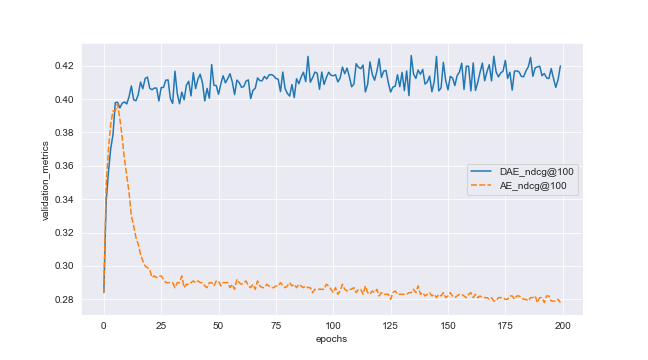
\includegraphics[width=1\textwidth]{ndcg_AEvsDAE_ML20.png}
        \caption[Độ đo NDCG trên tập kiểm tra của mô hình AE trên tập dữ liệu MovieLens]{Độ đo NDCG@100 trên tập dữ liệu kiểm định của bộ dữ liệu MovieLens của hai mô hình AE khi áp dụng ``dropout'' và không sử dụng ``dropout''}
        \label{ndcg_AE_ML20}
    \end{figure}

    \begin{figure}
        \centering
        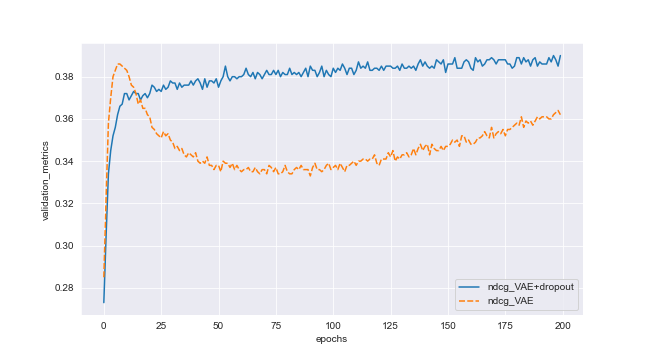
\includegraphics[width=1\textwidth]{ndcg_VAE_ML20.png}
        \caption[Độ đo NDCG trên tập kiểm tra của mô hình VAE trên tập dữ liệu MovieLens]{Độ đo NDCG@100 trên tập dữ liệu kiểm định của bộ dữ liệu MovieLens của hai mô hình VAE khi áp dụng ``dropout'' và không sử dụng ``dropout''}
        \label{ndcg_VAE_ML20}
    \end{figure}


    \subsection{Phân tích ``Multinomial Likelihood''}

    Ở phần này, chúng tôi sẽ trình bày thí nghiệm để kiểm chứng hàm lỗi Multinomial log-likelihood so với các hàm lỗi thường được dùng khác.
    Cụ thể chúng tôi sẽ so sánh Multinomial log-likelihood so với Gaussian log-likelihood và Logistic log-likelihood. 


    Hàm ``Multinomaial log-likelihood'' như đã được trình bày ở phần \ref{mulll} sẽ giả định dữ liệu ban đầu sẽ được phát sinh bởi một phân phối đa thức (``Multinomial Distribution'').
    Và kết quả trả về của mô hình Mult-VAE là một véc-tơ thể hiện xác suất được chọn của từng sản phẩm trong hệ thống (véc-tơ này có tổng bằng 1).
    
    Về Gaussian log-likelihood, cũng chính là độ lỗi ``Mean Square Error'', là một độ lỗi thường gặp trong những bài toán hồi quy (regression). 
    Với độ lỗi này thì dữ liệu tương tác của người dùng được giả định sẽ tuân theo phân phối Gaussian. 
    Theo đó, chúng tôi dựa vào bài báo \cite{yifan_cf} của tác giả Yifan Hu, đã áp dụng Gaussian log-likelihood cho bài toán gợi ý sản phẩm với dữ liệu ``implicit feedback''. 
    Theo bài báo thì Gaussian log-likelihood cho người dùng $u$ sẽ là:
    \begin{equation}
        \log p_\theta(x_u|z_u) = -\sum_i \frac{c_{ui}}{2}(x_{ui} - f_{ui})^2
    \end{equation}
    trong đó, $c_{ui}$ là hệ số ``confidence'' của tương tác được thực hiện bởi người dùng $u$ với sản phẩm $i$ và $f_{ui}$ là kết quả tái tạo lại tương tác của người dùng $u$ với sản phẩm $i$.
    Hệ số ``confidence'' $c_{ui}$ kiểm soát sự ảnh hưởng giữa những sản phẩm được tương tác với những sản phẩm không được tương tác.
    Cụ thể, những sản phẩm được tương tác sẽ có giá trị hệ số ``confidence'' cao hơn so với những sản phẩm không tương tác.
    Có nghĩa là $c_{1}  > c_0$, với $c_1,c_0$ lần lượt là hệ số ``confidence'' của sản phẩm được tương và sản phẩm không được tương tác. 
    
    Bên cạnh đó, Logistic log-likelihood, hay còn được biết đến là độ lỗi ``Binary cross entropy'', là một độ lỗi thường được dùng trong những bài toán phân loại (classification).
    Về lý thuyết xác suất, sử dụng mô hình này ta sẽ giả định rằng dữ liệu của chúng ta sẽ được phát sinh từ một phân phối Bernoulli. 
    Với việc sử dụng, Logistic log-likelihood thì bài toán xây dựng hệ thống gợi ý sản phẩm hay cụ thể việc xác định tương tác của một người dùng với một sản phẩm sẽ được xem như bài toán phân loại 2 lớp. 
    Logistic log-likelihood của người dùng u sẽ được tính như sau:
    \begin{equation}
        \log p_\theta(x_u|z_u) = -\sum_i x_{ui}\log \sigma(f_{xui}) + (1-x_{ui})\log(1 - \sigma(f_{ui}))
    \end{equation}
    Trong đó $\sigma(x) = \frac{1}{1+\exp (-x)}$ là hàm logistic và  $f_{ui}$ là kết quả tái tạo lại tương tác của người dùng $u$ với sản phẩm $i$.
    Để thể hiện sự hiệu quả của multinomial log-likelihood so với hai hàm lỗi còn lại trong bài toán gợi ý sản phẩm với sản phầm phản hồi ngầm, chúng tôi lần lượng thực hiện huấn luyện mô hình với các độ lỗi trên và ghi lại kết quả tốt nhất. 
    Trong thí nghiệm này việc huấn luyện mô hình chỉ thay đổi độ lỗi và các thiết lập khác sẽ được giữ nguyên.
    Cụ thể, chúng tôi tiến hành thay đổi hàm lỗi ``Multinomial log-likelihood'' thành các hàm lỗi ``Gaussian likelihood'' và ``Logistic log-likelihood'' trên hai mô hình ``Variational Auto-encoder'' và ``Auto-encoder'' với các thiết lập giống phần~\ref{setup_experiment}.
    Và chúng tôi thực hiện ``fine-tune'' siêu tham số tách biệt giữa các độ lỗi với nhau.
    Vì tính chất của ``Multinomial log-likelihood'' phục vụ mục đích xếp hạng các sản phẩm ``phù hợp'' với người dùng, do đó chúng tôi dùng độ đo Normalized Discounted Cumulative Gain (NDCG) để đánh giá chất lượng xếp hạng của mô hình. 
    
    Kết quả thực nghiệm được ghi nhận lại ở bảng~\ref{table:comparell} thể hiện độ đo NDCG@100 với các hàm lỗi và mô hình tương ứng. 
    Từ kết quả cho ta thấy ảnh hưởng của ``Multinomial log-likelihood'' lên chất lượng xếp hạng của mô hình (đánh giá thông qua độ đo NDCG@100). 
    Điều này chứng tỏ được rằng việc lựa chọn hàm lỗi thực sự phụ thuộc vào dữ liệu của mô hình. 
    Và đối với bài toán gợi ý sản phẩm, cụ thể là với dữ liệu phản hồi ngầm thì multinomial log-likelihood mang lại kết quả ấn tượng. 
    Từ đó cho thấy ``Multinomial log-likelihood'' là một hàm lỗi phù hợp với hệ thống gợi ý, khi chúng ta muốn ``xếp hạng'' các sản phẩm, từ đó đưa ra các gợi ý tốt nhất cho người dùng.            

    \begin{table}[]
    \centering
        \begin{tabular}{|c|c|c|c|}
        \hline
                        & \textbf{Multinomial}                  & \textbf{Gaussian}            & \textbf{Logistics}           \\ \hline
        \textbf{VAE} &  \textbf{0.429} & 0.422 &  0.419 \\ \hline
        \textbf{DAE}  & \textbf{0.423}                        & 0.409                        & 0.412                        \\ \hline
        \end{tabular}
    
    \caption[Kết quả mô hình với các hàm lỗi khác nhau]{Độ đo NDCG@100 trên các mô hình VAE và DAE với các hàm lỗi khác nhau trên tập dữ liệu MovieLens}
    \label{table:comparell}
    \end{table}   
   
   \subsection{Phân tích sự đánh đổi trong hàm ELBO}
   Như đã trình bày ở phần \ref{subsubsecELBO} thì trong hàm ELBO, hàm mục tiêu trong quá trình huấn luyện ``Variational Auto-Encoder'', có tồn tại một sự đánh đổi.
   Đó là sự đánh đổi giữa việc mô hình hóa dữ liệu và việc đặc trưng ẩn được phát sinh tuân theo phân phối xác suất đã được giả định trước trong việc huấn luyện mô hình.
   Và chúng tôi đã đưa ra khẳng định rằng trong bài toán xây dựng gợi ý sản phẩm thì ta sẽ quan tâm đến khả năng mô hình hoá nhiều hơn là việc đảm bảo đặc trưng ẩn tuân theo một phân phối xác suất.
   Do đó, ở mục này chúng tôi sẽ tiến hành kiểm chứng lại điều này.

   Chúng tôi thực hiện huấn luyện mô hình ``Variational Auto-Encoder'' với hai độ lỗi khác nhau, tương ứng với hàm ELBO thông thường (công thức \ref{elbo_mvae}) và hàm ELBO với tham số $\beta$ (công thức \ref{elbo_betamvae}) để kiểm soát sự đánh đổi nói trên.
   Để thống nhất thì chúng tôi sẽ huấn luyện một mô hình với kĩ thuật ``KL-annealing'' (được trình bày ở mục \ref{subsubsecELBO}) và một mô hình với giá trị $\beta =1$ cố định.
   Với $\beta = 1$ thì ta có được hàm ELBO thông thường, do đó thí nghiệm này nhằm mục đích để kiểm chứng sự ảnh hưởng của siêu tham số $\beta$ trong bài toán xây dựng hệ thống gợi ý sản phẩm.
   Với kĩ thuật ``KL-annealing'' chúng tôi sẽ để giới hạn cho mô hình là 0.2, có nghĩa là $\beta$ được tăng dần từ 0 đến 0.2.
   Giá trị giới hạn được lựa chọn dựa trên những thực nghiệm trước đó, chung tôi dựa vào những lần huấn luyện trước đó và nhận thấy rằng giới hạn $\beta$ bằng 0.2 cho kết quả mô hình tốt nhất.
   %Ngoài ra với tập dữ liệu MSD thì chúng tôi còn thực hiện thêm việc huấn luyện mô hình với giá trị giới hạn của $\beta = 1$.
   %Nhằm mục có thể thể hiện rõ hơn sự ảnh hưởng của giá trị của siêu tham số $\beta$
   Quá trình huấn luyện sẽ được thực hiện như các thiết lập đã trình bày ở mục \ref{setup_experiment}.
   Việc đánh giá dựa trên độ đo NDCG@100 ở tập đánh giá (validation) và được thực hiện trên cả hai tập dữ liệu MovieLens và Million Song Datasets. 
   
   \begin{figure}
    \centering
    \includegraphics[width=1\textwidth]{movilen_beta.png}
    \caption[Mô hình Mult-VAE trong việc kiểm soát siêu tham số]{So sánh Mult-VAE trong việc kiểm soát tham sự đánh đổi giữa khả năng mô hình hóa và việc đặc trưng ẩn tuân theo phân phối xác suất trên tập MovieLens}
    \label{beta_movielen}
    \end{figure}

    Hình \ref{beta_movielen} thể hiện kết quả khi huấn luyện mô hình trên tập dữ liệu MovieLens.
    Ta dễ dàng thấy được rằng, khi thực hiện huấn luyện mô hình với hàm ELBO thông thường ($\beta=1$ tương ứng với hàm ELBO thông thường) thì cho kết quả thấp hơn hẳn so với phiên bản có sự kiểm soát của siêu tham số $\beta$.
    Với những epoch đầu, thì cách biệt không quá lớn và cũng k ổn định, tuy nhiên sau một số lượng epoch nhất định thì cách biệt này dần trở nên rõ rệt hơn.

    \begin{figure}
        \centering
        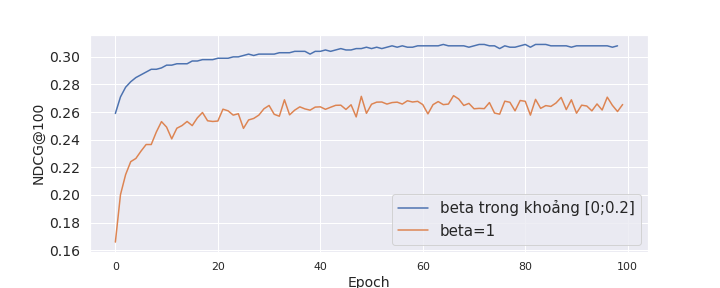
\includegraphics[width=1\textwidth]{msd_beta.png}
        \caption[Mô hình Mult-VAE trong việc kiểm soát siêu tham số]{So sánh Mult-VAE trong việc kiểm soát tham sự đánh đổi giữa khả năng mô hình hóa và việc đặc trưng ẩn tuân theo phân phối xác suất trên tập MSD}
        \label{beta_msd}
    \end{figure}


    
    Hình \ref{beta_msd} thể hiện kết quả khi thí nghiệm trên tập dữ liệu MSD. 
    Ở tập dữ liệu này ta có thể thấy rõ ràng sự khác biệt trong việc kiểm soát siêu tham số $\beta$.
    Theo đó, ta dễ dàng thấy được ngay từ những epoch đầu, với hàm ELBO thông thường sẽ cho kết quả cực kỳ thấp. 
    Ngược lại với việc có siêu tham số $\beta$ kiểm soát thì kết quả ngày từ những epoch đầu cũng đã vượt trội hơn và phần nào mô hình cũng ổn định hơn. 

    Qua kết quả trên, ta có thể thấy được rằng trong bài toán xây dựng hệ thống gợi ý sản phẩm thì việc có sự kiểm soát giữa khả năng mô hình hóa dữ liệu của mô hình và việc đặc trưng ẩn được phát sinh là một yếu tố quan trọng để xây dựng một hệ thống gợi ý sản phẩm hiệu quả.



   
    \subsection{``Variational Auto-encoder'' và ``Auto-encoder'' đối với trường hợp dữ liệu thưa}
    Trong phần này, mục tiêu của  chúng tôi là kiểm chứng về sự phù hợp của ``Variational Auto-encoder'' so với ``Auto-encoder'', cụ thể là so sánh Mult-VAE và Mult-DAE.
    Theo góc nhìn khác thì ta có thể xem như đây là thí nghiệm so sánh giữa phương pháp ``Bayesian inference'' cho đặc trưng ẩn là một phân bố so với hướng tiếp cận xấp xỉ đặc trưng ẩn là một điểm xác định.

    Như đã trình bày ở mục \ref{why_vae}, thì mô hình Mult-VAE được xây dựng dựa trên các giả định của chúng tôi về dữ liệu, cụ thể là khi dữ liệu thưa.
    Do đó chúng tôi sẽ đánh giá hai mô hình Mult-VAE với tình trạng dữ liệu thưa.

    Theo thí nghiệm ở mục \ref{experiment1} thì ta có thể thấy được ở tập MovieLens thì cách biệt giữa Mult-VAE và Mult-DAE là lớn hơn so với tập MSD.
    Để kiểm chứng hiệu quả của Mult-VAE tốt hơn Mult-DAE ở điều kiện dữ liệu thưa, ở thí nghiệm này, cụ thể thì trong tập kiểm tra chúng tôi sẽ lần lượt thí hiện giảm số lượng tương tác người dùng trong tập ``fold-in'' (ở đánh giá trước các đánh giá dựa trên tập ``fold-in'' gồm 80\% tương tác của người dùng). Và đánh giá kết quả của mô hình dựa trên số lượng tương tác còn lại.
    
    \begin{figure}
        \centering
        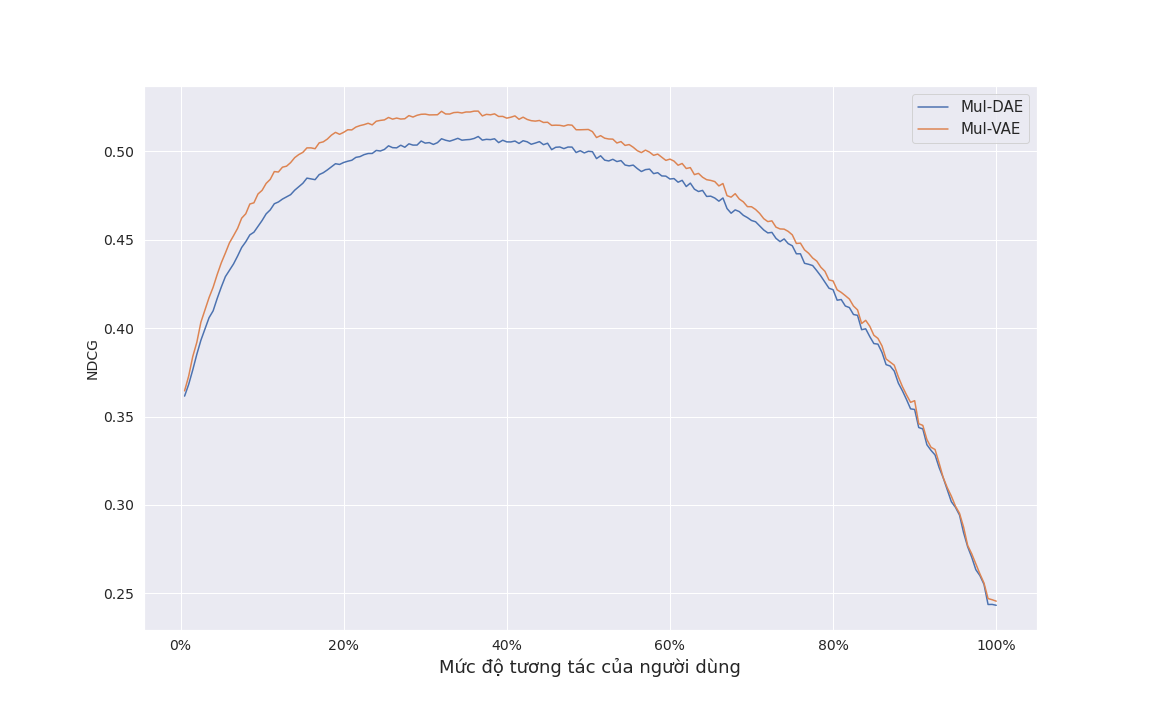
\includegraphics[width=1\textwidth]{vae_dae_ml.png}
        \caption[So sánh Mult-VAE và Mult-DAE trên tập MovieLens]{So sánh Mult-VAE và Mult-DAE ở các mức độ tương tác khác nhau trên tập kiểm tra trên tập MovieLens}
        \label{fig_vae_dae_ml}
    \end{figure}
    \begin{figure}
        \centering
        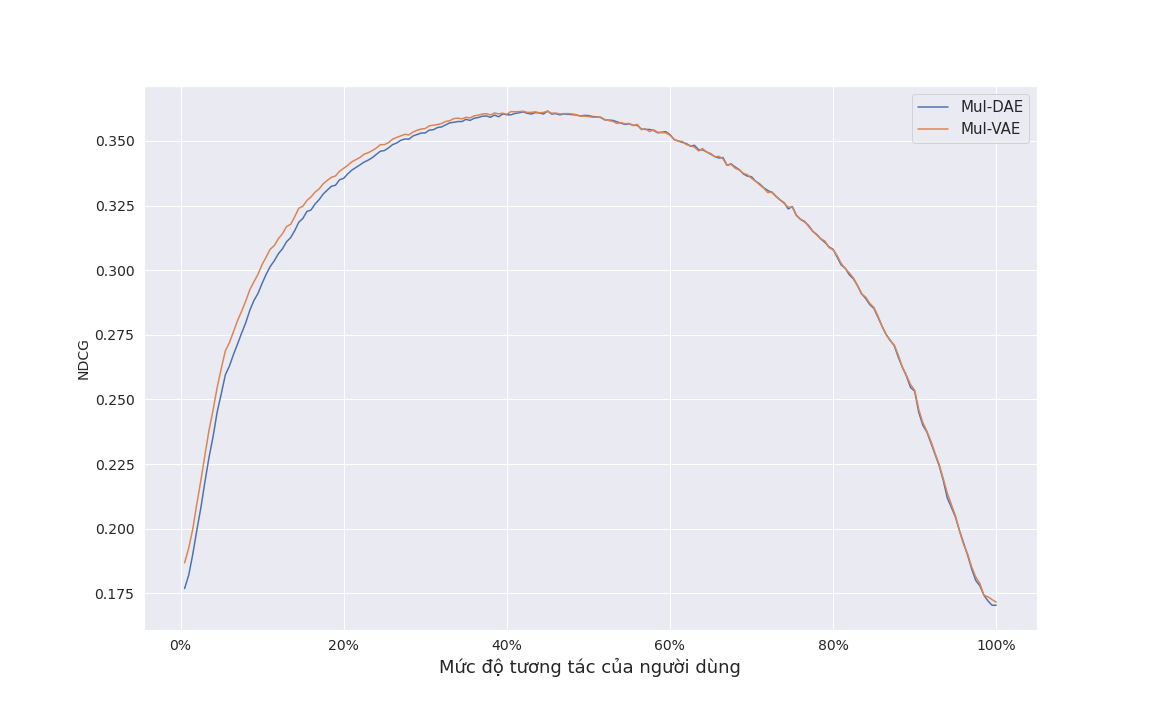
\includegraphics[width=1\textwidth]{vae_dae_msd.png}
        \caption[So sánh Mult-VAE và Mult-DAE trên tập MSD]{So sánh Mult-VAE và Mult-DAE ở các mức độ tương tác khác nhau trên tập kiểm tra trên tập Million Song Datasets}
        \label{fig_vae_dae_msd}
    \end{figure}

    Hình \ref{fig_vae_dae_ml} thể hiện giá trị của độ đo NDCG@100 trên tập MovieLens. 
    Với tập dữ liệu này, ta dễ dàng nhận thấy Mult-VAE vượt trội hơn so với Mult-DAE, đặc biệt là khi dữ liệu tương tác người dùng thấp.
    Cụ thể trong khoảng mức độ tương tác của người dùng từ 20\% đến 40\% thì Mult-DAE hoàn toàn bị bỏ xa bởi Mult-VAE.
    Hình \ref{fig_vae_dae_msd} là kết quả thực hiện thí nghiệm trên tập MSD.
    Tập dữ liệu này cũng có xu hướng tương tự như trên tập MovieLens, tuy nhiên sự cách biệt giữa Mult-DAE và Mult-VAE không quá rõ ràng.
    Song, ta vẫn dễ dàng nhận thấy được rằng với mức độ tương tác thấp Mult-VAE vẫn cho kết quả nhỉnh hơn so với Mult-DAE.

    Kết quả thí nghiệm giúp ta đã giúp khẳng định lại được độ hiệu quả của mô hình Mult-VAE được đề xuất trong bài báo \cite{mvae}. 
    Tuy trên tổng quan thì Mult-VAE không quá vượt trội so với Mult-DAE nhưng ở trường hợp dữ liệu tương tác người dùng ở mức độ thấp thì Mult-VAE mang lại kết quả cực kỳ ấn tượng.
